%%%%%%%%%%%%%%%%%%%%%%%%%%%%%%%%%%%%%%%%%
% Beamer Presentation
% LaTeX Template
% Version 1.0 (10/11/12)
%
% This template has been downloaded from:
% http://www.LaTeXTemplates.com
%
% License:
% CC BY-NC-SA 3.0 (http://creativecommons.org/licenses/by-nc-sa/3.0/)
%
%%%%%%%%%%%%%%%%%%%%%%%%%%%%%%%%%%%%%%%%%

%----------------------------------------------------------------------------------------
%	PACKAGES AND THEMES
%----------------------------------------------------------------------------------------

\documentclass[10pt]{beamer}

\mode<presentation> {

% The Beamer class comes with a number of default slide themes
% which change the colors and layouts of slides. Below this is a list
% of all the themes, uncomment each in turn to see what they look like.

%\usetheme{default}
%\usetheme{AnnArbor}
%\usetheme{Antibes}
%\usetheme{Bergen}
%\usetheme{Berkeley}
%\usetheme{Berlin}
%\usetheme{Boadilla}
%\usetheme{CambridgeUS}
%\usetheme{Copenhagen}
%\usetheme{Darmstadt}
%\usetheme{Dresden}
\usetheme{Frankfurt}
%\usetheme{Goettingen}
%\usetheme{Hannover}
%\usetheme{Ilmenau}
%\usetheme{JuanLesPins}
%\usetheme{Luebeck}
%\usetheme{Madrid}
%%\usetheme{Malmoe}
%\usetheme{Marburg}
%\usetheme{Montpellier}
%\usetheme{PaloAlto}
%\usetheme{Pittsburgh}
%\usetheme{Rochester}
%\usetheme{Singapore}
%\usetheme{Szeged}
%\usetheme{Warsaw}

% As well as themes, the Beamer class has a number of color themes
% for any slide theme. Uncomment each of these in turn to see how it
% changes the colors of your current slide theme.

%\usecolortheme{albatross}
%\usecolortheme{beaver}
%\usecolortheme{beetle}
%\usecolortheme{crane}
%\usecolortheme{dolphin}
%\usecolortheme{dove}
%\usecolortheme{fly}
%\usecolortheme{lily}
%\usecolortheme{orchid}
%\usecolortheme{rose}
%\usecolortheme{seagull}
%\usecolortheme{seahorse}
%\usecolortheme{whale}
%\usecolortheme{wolverine}

%\setbeamertemplate{footline} % To remove the footer line in all slides uncomment this line
\setbeamertemplate{footline}[page number] % To replace the footer line in all slides with a simple slide count uncomment this line

%\setbeamertemplate{navigation symbols}{} % To remove the navigation symbols from the bottom of all slides uncomment this line
}

\newcommand{\cmd}[1]{\\\texttt{#1}\\}
\newcommand{\cmduser}[1]{\texttt{\$ #1}\\}
\newcommand{\cmdroot}[1]{\\\texttt{\# #1}\\}
\usepackage{graphicx} % Allows including images
\usepackage{booktabs} % Allows the use of \toprule, \midrule and \bottomrule in tables
\usepackage[italian]{babel}
\usepackage[utf8]{inputenc}
\usepackage[T1]{fontenc}
\usepackage{lmodern}
\usepackage{minted}
\usepackage{tikz}
\usetikzlibrary{shapes,shadows,arrows}
%\usepackage{fancyhdr}
\usepackage{epigraph}
\setlength{\epigraphwidth}{33em}
%\usepackage{float}
%\restylefloat{table}
\usepackage{url}
\usepackage{hyperref}
%\usefonttheme{professionalfonts}
%\usepackage{lxfonts}
\beamertemplatetransparentcovereddynamic
%\usefonttheme[default]{professionalfonts} % structureitalicserif,structureitalicserif
%\usepackage[bookmarks,pdftex,
%pdfauthor={Francesco Soncina},
%pdftitle={IEEE 802.21: Media Independent Handover},
%pdfsubject={IEEE 802.21},
%pdfkeywords={IEEE, 802.21, ODTONE, MIHF},
%pdfproducer={Latex with hyperref},
%pdfcreator={pdflatex}]{hyperref}


%----------------------------------------------------------------------------------------
%	TITLE PAGE
%----------------------------------------------------------------------------------------

\title[IEEE 802.21]{IEEE 802.21: Media Independent Handover} % The short title appears at the bottom of every slide, the full title is only on the title page

\author{Francesco Soncina} % Your name
%\institute[] % Your institution as it will appear on the bottom of every slide, may be shorthand to save space
{
%University of California \\ % Your institution for the title page
%\medskip
%\textit{xxx@gmail.com} % Your email address
}
\date{Bologna, 18 Marzo 2014\\\vspace{1.5em}Tesi di Laurea in Informatica}
\begin{document}
\begin{frame}
\titlepage % Print the title page as the first slide
\begin{minipage}[t]{0.47\textwidth}
Relatore:\\
Chiar.mo Prof.\\
Vittorio Ghini
\end{minipage}
\hfill
\begin{minipage}[t]{0.47\textwidth}\raggedleft
Presentata da:\\
Francesco Soncina
\end{minipage}
\end{frame}

\begin{frame}
\frametitle{Indice} % Table of contents slide, comment this block out to remove it
\tableofcontents % Throughout your presentation, if you choose to use \section{} and \subsection{} commands, these will automatically be printed on this slide as an overview of your presentation
\end{frame}

%----------------------------------------------------------------------------------------
%	PRESENTATION SLIDES
%----------------------------------------------------------------------------------------

%------------------------------------------------
\section{Introduzione} % Sections can be created in order to organize your presentation into discrete blocks, all sections and subsections are automatically printed in the table of contents as an overview of the talk
%------------------------------------------------

\subsection{Tipi di handovers}
\begin{frame}
\frametitle{Tipi di handovers}
L'{\em Handover} è l'atto di cambiare l'{\em access point} al fine di mantenere la connettività e può essere catalogato secondo due differenti criteri:
\begin{enumerate}
\item Tecnologia prima e dopo il passaggio
\begin{itemize}
\item Horizontal handover (intra-rat): la tecnologia a livello {\em data link} non cambia (e.g. WiFi $\to$ WiFi)
\item Vertical handover (inter-rat): la tecnologia a livello {\em data link} cambia (e.g. WiFi $\to$ LTE)
\end{itemize}

\item Stato della sessione prima e dopo il passaggio
\begin{itemize}
\item Hard handover (break-before-make): tutte le connessioni aperte vengono interrotte prima di effettuare il passaggio
\item Soft handover (make-before-break):  le connessioni vengono ristabilite attraverso il nuovo {\em link} prima di chiudere le precedenti
\end{itemize}
\end{enumerate}
\end{frame}

\subsection{Graficamente}
\begin{frame}
\frametitle{Graficamente}
\begin{figure}[h!]
\centering
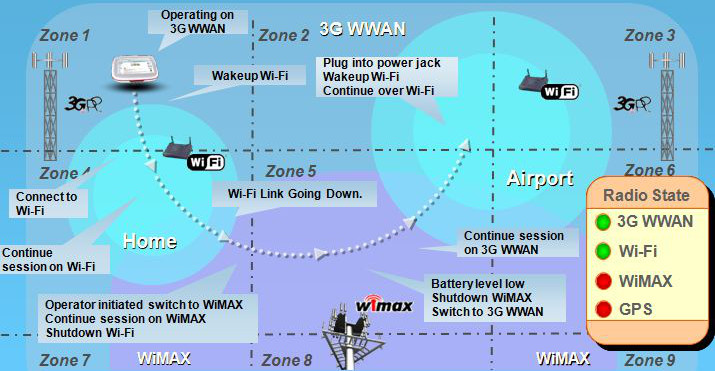
\includegraphics[scale=0.4]{handovers.jpg}
\caption{Esempi di {\em handovers}}
\label{fig:handovers}
\end{figure}
\end{frame}

\subsection{Problematiche}
\begin{frame}
\frametitle{Problematiche}
Ogni giorno ci sono sempre più {\em devices} dotati di più interfacce di rete e quindi la gestione del processo di {\em handover} è diventata sempre più importante. I principali problemi da gestire sono:
\begin{enumerate}
\item Decisioni di handover (IEEE 802.21)
\item Mantenimento sessione in handovers nella stessa rete (IEEE 802.11r-2008)
\item Mantenimento sessione in handovers tra reti diverse (IETF Mobile IPv4/IPv6)
\end{enumerate}
\end{frame}

%\begin{columns}[c] % The "c" option specifies centered vertical alignment while the "t" option is used for top vertical alignment
%\column{.45\textwidth} % Left column and width
%\textbf{Heading}
%\begin{enumerate}
%\item Statement
%\item Explanation
%\item Example
%\end{enumerate}
%\column{.5\textwidth} % Right column and width
%Lorem ipsum dolor sit amet, consectetur adipiscing elit. Integer lectus nisl, ultricies in feugiat rutrum, %porttitor sit amet augue. Aliquam ut tortor mauris. Sed volutpat ante purus, quis accumsan dolor.
%\end{columns}

\section{Standard IEEE 802.21}
\subsection{Finalità}
\begin{frame}
\frametitle{Finalità}
Lo standard IEEE 802.21 si assume l'onere di risolvere il primo dei precedenti problemi, ovvero come debbano avvenire le decisioni di {\em handover}, in particolare:
\begin{itemize}
\item recupero delle informazioni necessarie sullo stato dei vari collegamenti disponibili: specifica tutti i servizi necessari per acquisire informazioni utili sullo stato delle interfacce per facilitare le future azioni di {\em handover}
\item propagazione di eventi e comandi alle entità interessate: gestisce lo smistamento dei messaggi verso le entità interessate, per comunicare ad un utente degli eventi oppure per impartire dei comandi ad un'interfaccia, al fine di facilitare il passaggio
\item logica di funzionamento {\em media-independent}: è possibile per specifica ottenere informazioni su tutti i tipi di interfacce, senza differenze per tecnologia adottata.
\end{itemize}
\end{frame}

\subsection{Architettura}
\begin{frame}
\frametitle{Architettura}
Le entità previste dallo standard sono:
\begin{enumerate}
\item {\em Media Independent Handover Function} (MIHF): è il {\em core} dello standard
\begin{itemize}
\item Media Independent Event Services (MIES): gestisce propagazione eventi
\item Media Independent Command Services (MICS): gestisce propagazione comandi
\item Media Independent Information Services (MIIS): gestisce propagazione {\em queries} e relative risposte
\end{itemize}

\item {\em Link\_Sap}: forniscono dei servizi ad un MIHF (e.g. generazione di eventi, esecuzione di comandi, etc)
\begin{itemize}
\item {\em media-specific}: gestiscono solo una tipologia di interfaccia
\item {\em media-independent}: forniscono un'astrazione generale per ogni tipo di interfaccia
\end{itemize}

\item {\em MIH-User}: è l'entità che sfrutta i servizi offerti da un MIHF.

\end{enumerate}
\end{frame}

\section{ODTONE}
\subsection{Funzionalità implementate}
\begin{frame}
\frametitle{Funzionalità implementate}
ODTONE è una implementazione dello standard IEEE 802.21 {\em open-source} (LGPLv3), resa {\em cross-platform} attraverso la libreria Boost (eseguibile su sistemi GNU/Linux, Windows, Android ed OpenWrt) e fornisce:

\begin{itemize}

\item MIHF: fornisce un'implementazione del core e supporta la propagazione di ogni tipo di evento e comando
\item Link\_Sap generico: è compatibile con ogni famiglia di interfacce, ma supporta solo eventi {\em Link\_Up} e {\em Link\_Down}
\item Link\_Sap specifico per 802.3/802.11: supporta più eventi e comandi, ma solo per 802.3 e 802.11
\item MIH-User: fornisce un esempio di applicazione utente che possa comunicare con l'MIHF
\item libodtone: è la libreria ufficiale per interagire correttamente con ODTONE a livello applicativo
\end{itemize}


\end{frame}
\subsection{Pro e contro}
\begin{frame}
\frametitle{Pro e contro}
\begin{block}{Pro}

\begin{itemize}
\item cross-platform
\item open-source
\item facilmente espandibile
\item il core supporta la propagazione di tutti gli eventi e comandi
\end{itemize}
\end{block}

\begin{block}{Contro}
\begin{itemize}
\item il SAP generico genera solo gli eventi {\em Link\_Up} e {\em Link\_Down}
\item sono forniti SAP specifici solo per 802.3 e 802.11
\item i SAP specifici non implementano tutti gli eventi e comandi previsti
\item non sono forniti SAP per nessuna tecnologia della famiglia 3GPP
\end{itemize}
\end{block}
\end{frame}

\section{MIH-proxy}
\subsection{Obbiettivi}
\begin{frame}
\frametitle{Obbiettivi}
Per poter testare sia lo standard IEEE 802.21 sia l'implementazione ODTONE è stata realizzata un'applicazione in grado di rimanere in ascolto degli eventi generati dall'MIHF al fine di realizzare un proxy ad alta affidabilità, i.e. in grado di utilizzare più interfacce di rete per gestire una singola connessione, ed è stato realizzato in due versioni:
\begin{itemize}
\item \textbf{Simplex}: è in grado di gestire una comunicazione di sola uscita, sfruttando le interfacce disponibili secondo la politica di {\em scheduling} adottata. (il destinatario non deve considerare l'IP sorgente)
\item \textbf{Full-duplex}: è in grado di gestire una comunicazione bidirezionale, sfruttando le interfacce disponibili sia per ricevere sia per inviare, per entrambi i {\em peers}.
\end{itemize}

%\begin{block}{Block 1}
%Lorem ipsum dolor sit amet, consectetur adipiscing elit. Integer lectus nisl, ultricies in feugiat rutrum, %porttitor sit amet augue. Aliquam ut tortor mauris. Sed volutpat ante purus, quis accumsan dolor.
%\end{block}
\end{frame}

\subsection{Graficamente}
\begin{frame}
\frametitle{Graficamente}
\begin{figure}[h!]
\centering
\begin{tikzpicture}
\tikzset{
block/.style={rectangle,rounded corners,draw=black, top color=white, bottom color=gray!50,very thick, node distance=3.5em},
%inner sep=1em, minimum size=1em, text centered,node distance=3em},
mynode/.style={rectangle,fill=gray!30, text centered, text width=2em,minimum height=2mm,node distance=1em},
myarrow/.style={->, >=latex', shorten >=1pt, very thick},
mydoublearrow/.style={<->, >=latex', shorten >=1pt, very thick},
dottedarrow/.style={<->, >=latex', shorten >=1pt, thick, dotted},
mylabel/.style={text width=1em, text height=1em, text centered},
}

\node [block] (client) {Client};
\node [block, below of=client] (mihproxy1) {MIH-proxy};
\node [block, below of=mihproxy1] (mihf) {MIHF};
\node [block, below of=mihf, xshift=-4em] (linksap1) {MIH-Link-Sap};
\node [block, below of=mihf, xshift=4em] (linksap2) {MIH-Link-Sap};
\node [block, below of=linksap1] (eth0) {eth0};
\node [block, below of=linksap2] (wlan0) {wlan0};
\node [block, right of=client, xshift=8em] (server) {Server};
\draw[myarrow] (client) -- node[auto,swap] {UDP} (mihproxy1);
\draw[dottedarrow] (mihproxy1) -- (mihf);
\draw[dottedarrow] (mihf) -- (linksap1);
\draw[dottedarrow] (mihf) -- (linksap2);
\draw[dottedarrow] (linksap1) -- (eth0);
\draw[dottedarrow] (linksap2) -- (wlan0);
\draw[myarrow] (mihproxy1) -- ++(3,0) |-  (wlan0);
\draw[myarrow] (mihproxy1) -- ++(-3,0) |-  (eth0);
\draw[myarrow] (eth0.south) -- ++(0,-1) -|  (server.south);
\draw[myarrow] (eth0.south) -- ++(0,-1) -|  (server.south);
\draw[myarrow] (wlan0.south) -- ++(0,-1) -| (server.south);
\end{tikzpicture}
\caption{MIH-proxy unidirezionale}
\label{fig:mihproxyuni}
\end{figure}
\end{frame}

\begin{frame}
\frametitle{Graficamente}

\begin{figure}[h!]
\centering
\begin{tikzpicture}
\tikzset{
block/.style={rectangle,rounded corners,draw=black, top color=white, bottom color=gray!50,very thick, node distance=3.5em},
%inner sep=1em, minimum size=1em, text centered,node distance=3em},
mynode/.style={rectangle,fill=gray!30, text centered, text width=2em,minimum height=2mm,node distance=1em},
myarrow/.style={->, >=latex', shorten >=1pt, very thick},
mydoublearrow/.style={<->, >=latex', shorten >=1pt, very thick},
dottedarrow/.style={<->, >=latex', shorten >=1pt, thick, dotted},
mylabel/.style={text width=1em, text height=1em, text centered},
}

\node [block] (client) {Client};
\node [block, below of=client] (phoxy1) {phoxy};
\node [block, below of=phoxy1] (mihproxy1) {MIH-proxy};
\node [block, below of=mihproxy1] (mihf1) {MIHF};
\node [block, below of=mihf1, xshift=-3.0em] (linksap1) {Link-Sap};
\node [block, below of=mihf1, xshift=3.0em] (linksap2) {Link-Sap};
\node [block, below of=linksap1] (eth0) {eth0};
\node [block, below of=linksap2] (wlan0) {wlan0};
\node [block, right of=client, xshift=11em] (server) {Server};
\node [block, below of=server] (phoxy2) {phoxy};
\node [block, below of=phoxy2] (mihproxy2) {MIH-proxy};
\node [block, below of=mihproxy2] (mihf2) {MIHF};
\node [block, below of=mihf2, xshift=-3.0em] (linksap3) {Link-Sap};
\node [block, below of=mihf2, xshift=3.0em] (linksap4) {Link-Sap};
\node [block, below of=linksap3] (eth01) {eth0};
\node [block, below of=linksap4] (eth11) {eth1};
\draw[mydoublearrow] (client) -- node[auto,swap] {TCP} (phoxy1);
\draw[mydoublearrow] (phoxy1) -- node[auto,swap] {UDP+AES} (mihproxy1);
\draw[dottedarrow] (mihf1) -- (linksap1);
\draw[dottedarrow] (mihf1) -- (linksap2);
\draw[dottedarrow] (mihproxy1) -- (mihf1);
\draw[dottedarrow] (linksap1) -- (eth0);
\draw[dottedarrow] (linksap2) -- (wlan0);
\draw[mydoublearrow] (mihproxy1) -- ++(2.3,0) |- (wlan0);
\draw[mydoublearrow] (mihproxy1) -- ++(-2.3,0) |- (eth0);
\draw[mydoublearrow] (server) -- node[auto,swap] {TCP} (phoxy2);
\draw[mydoublearrow] (phoxy2) -- node[auto,swap] {UDP+AES} (mihproxy2);
\draw[dottedarrow] (mihproxy2) -- (mihf2);
\draw[dottedarrow] (mihf2) -- (linksap3);
\draw[dottedarrow] (mihf2) -- (linksap4);
\draw[dottedarrow] (linksap3) -- (eth01);
\draw[dottedarrow] (linksap4) -- (eth11);
\draw[mydoublearrow] (mihproxy2) -- ++(2.3,0) |- (eth11);
\draw[mydoublearrow] (mihproxy2) -- ++(-2.3,0) |- (eth01);
\draw[mydoublearrow] (eth01.south) -- ++(0,-0.5) -| (eth0.south);
\draw[mydoublearrow] (eth11.south) -- ++(0,-0.5) -| (wlan0.south);
\end{tikzpicture}
\caption{MIH-proxy bidirezionale con phoxy}
\label{fig:mihproxybiphoxy}
\end{figure}
\end{frame}

\subsection{Internals}
\begin{frame} %[fragile] % Need to use the fragile option when verbatim is used in the slide
\frametitle{Internals}
\begin{itemize}
\item \textbf{Unidirezionale}: rimane in ascolto di eventi dell'MIHF per stabilire quali interfacce sono disponibili e invia tutto ciò che riceve dal client verso il server utilizzando potenzialmente anche più interfacce contemporaneamente, a seconda della politica di {\em scheduling} implementata. Gestisce solo pacchetti UDP, la comunicazione è in un sol verso e quindi basta una sola istanza dell'MIH-proxy.
\item \textbf{Bidirezionale}: rappresentato in figura \ref{fig:mihproxybiphoxy}, per poter trasferire traffico bidirezionale sono necessarie due istanze dell'MIH-proxy, i.e. una per {\em peer}. Questa versione è in grado di poter inviare i pacchetti a più destinatari attraverso più interfacce. Per sapere lo stato delle interfacce locali utilizza lo standard IEEE 802.21 mentre per lo stato delle interfacce del destinatario utilizza un sistema di {\em heartbeats} temporizzati. Per abilitare il supporto per flussi TCP è necessario aggiungere un altro programma, {\em phoxy}, incaricato di trasformare lo {\em stream} in datagrammi, gestire il loro rinvio in caso andassero persi, il loro riordinamento in caso arrivassero disordinati e può, a richiesta, cifrare i datagrammi con l'algoritmo a chiave simmetrica {\em AES256}.
\end{itemize}
\end{frame}

%------------------------------------------------
\section{Conclusione}
%------------------------------------------------
\subsection{Risultati e sviluppi futuri}
\begin{frame}
\frametitle{Risultati e sviluppi futuri}
\begin{itemize}
\item \textbf{Risultati}: dopo aver realizzato questa applicazione, è possibile dare un giudizio sia sullo standard IEEE 802.21 sia su ODTONE. Lo standard IEEE 802.21 si è dimostrato adeguato per fornire ai nodi mobili tutte le informazioni necessarie per gestire le decisioni di {\em handover}, nonostante il ristretto sottoinsieme di funzionalità che è stato possibile testare. ODTONE si è dimostrato una buona implementazione {\em open-source}, anche se tuttora in stato sperimentale, ed è stato efficace per realizzare l'applicazione proposta. 
\item \textbf{Sviluppi futuri}: nel prossimo futuro bisogna completare il corredo di {\em standards} necessari per eseguire effettivamente gli {\em handover} tra i vari tipi di tecnologie e completare il {\em deployment} di IEEE 802.21 in modo da renderlo pienamente utilizzabile nella realtà.
Per quanto riguarda ODTONE, la priorità è quella di aggiungere dei {\em Link\_SAP} specifici per le tecnologie mancanti, {\em in primis} quelle della famiglia 3GPP.
\end{itemize}
\end{frame}

\subsection{References}
\begin{frame}
\frametitle{References}
\footnotesize{
\begin{thebibliography}{99} % Beamer does not support BibTeX so references must be inserted manually as below

\bibitem[Repository, 2014]{repo} Repository di questo lavoro reperibile con i seguenti comandi:
\newblock \cmduser{git clone https://github.com/phra/802\_21.git}
oppure\\
\cmduser{wget https://github.com/phra/802\_21/archive/master.tar.gz}
\vspace{2em}
\bibitem[IEEE, 2008]{standard} IEEE 802.21 Working Group (2008)
\newblock IEEE 802.21: Media Independent Handover Services
\newblock \url{http://standards.ieee.org/getieee802/download/802.21-2008.pdf}

\bibitem[ODTONE Team]{odtone} ODTONE Team (2009-2014)
\newblock ODTONE
\newblock \url{http://atnog.github.io/ODTONE/}


\end{thebibliography}
}
\end{frame}

\end{document} 